\begin{figure}[htbp]
\centering
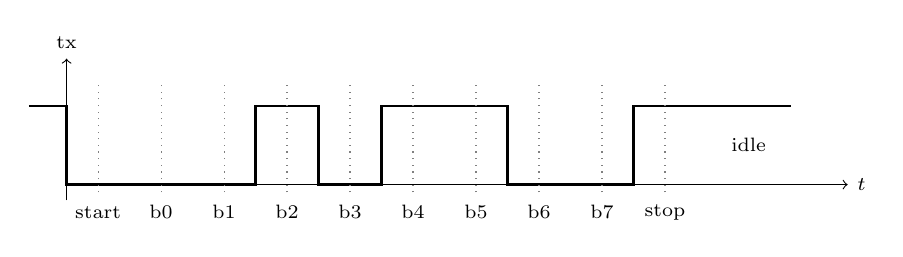
\begin{tikzpicture}[font=\footnotesize, x=8mm, y=10mm]
  % '4' = 0x34 = 0011 0100; 8N1 LSB first: start 0, bits 0,0,1,0,1,1,0,0, stop 1
  \draw[->] (0,0) -- (12.4,0) node[right]{\scriptsize $t$};
  \draw[->] (0,-0.2) -- (0,1.6) node[above]{\scriptsize tx};
  % bit cells: start 0-1, b0 1-2, b1 2-3, b2 3-4, b3 4-5, b4 5-6, b5 6-7, b6 7-8, b7 8-9, stop 9-10
  \draw[thick]
    (-0.6,1) -- (0,1) -- (0,0)   % idle high, falls at start bit
    -- (3,0) -- (3,1)            % start,b0,b1 low; b2 = 1 rises at 3
    -- (4,1) -- (4,0)            % b3 = 0
    -- (5,0) -- (5,1)            % b4 = 1
    -- (7,1) -- (7,0)            % b5 = 1, b6 = 0
    -- (9,0) -- (9,1)            % b7 = 0, stop = 1
    -- (11.5,1);
  \foreach \x/\b/\lbl in {0/0/start, 1/0/b0, 2/0/b1, 3/1/b2, 4/0/b3,
                          5/1/b4, 6/1/b5, 7/0/b6, 8/0/b7, 9/1/stop} {
    \node[font=\scriptsize] at (\x+0.5,-0.35) {\lbl};
    \draw[dotted,gray] (\x+0.5,-0.1) -- (\x+0.5,1.3);
  }
  \node[anchor=west] at (10.4,0.5) {\scriptsize idle};
\end{tikzpicture}
\caption{The wire-level frame the testbench observed for byte
0x34 (ASCII `4'): idle high, one start bit, eight data bits
LSB-first (\texttt{00110100} read right-to-left), one stop bit. Three
falling edges occur inside this one frame (the start bit and the
1-to-0 steps after b2 and b5), which is why a bench that counts
every falling edge on a four-byte message sees 13, not 4.}
\label{fig:uartwave08}
\end{figure}
